%
% phdtex
%
% Copyright (c) 2014-2020, Andrew Kanner <andrew.kanner@gmail.com>.
% All rights reserved.
%
% SPDX-License-Identifier: MIT
%

\documentclass[a5paper,10pt]{report}
% добавить leqno в [] для нумерации объектов слева
%\documentclass[a5paper,10pt,twoside]{report}

\IfFileExists{./template/contrib/styles.tex}{\def\template{./template}}{\def\template{.}}

% подключаемые пакеты, стили (в т.ч. ГОСТ Р 7.0.11-2011)
%%% Поля и разметка страницы %%%
\usepackage{lscape}		% Для включения альбомных страниц
\usepackage[headheight=17pt]{geometry}	% Для последующего задания полей (для устранения "\headheight is too small")

%%% Кодировки и шрифты %%%
\usepackage{cmap}						% Улучшенный поиск русских слов в полученном pdf-файле
\usepackage[T2A]{fontenc}				% Поддержка русских букв (кодировка)
\usepackage[utf8]{inputenc}				% Кодировка utf8 (исходного текста)
\usepackage[english, russian]{babel}	% Языки: русский, английский (локализация и переносы)
\usepackage{pscyr}						% Красивые русские шрифты
\usepackage{extsizes}					% Возможность сделать 14-й шрифт (не перенесено в documentclass extreport из-за неподдерживаемости в secsty)

%%% Альтернативные шрифты %%%
%\usepackage[english, russian]{babel}
%\usepackage{fontspec}					% загрузка шрифтов Open Type, True Type и др.
%\usepackage{euscript}					% Шрифт Евклид
%\usepackage{mathrsfs}					% Красивый матшрифт

%%% Оформление абзацев, колонтитулов, текста %%%
\usepackage{indentfirst}	% Красная строка
\frenchspacing
\usepackage{fancyhdr}		% Колонтитулы
\usepackage{setspace}		% Интерлиньяж

%%% Математические пакеты %%%
\usepackage{amsmath,amsfonts,amssymb,amsthm,mathtools,amscd}	% Математические дополнения от AMS
\usepackage{icomma}												% "Умная" запятая: $0,2$ --- число, $0, 2$ --- перечисление
\usepackage{mathtext}											% русские буквы в формулах
%\usepackage{leqno}												% Нумерация формул слева

%%% Цвета %%%
\usepackage[usenames]{color}
\usepackage{color}
\usepackage{colortbl}
\usepackage[usenames,dvipsnames,svgnames,table,rgb]{xcolor}

%%% Таблицы %%%
\usepackage{array,tabularx,tabulary,booktabs}	% Дополнительная работа с таблицами
\usepackage{longtable}							% Длинные таблицы
\usepackage{multirow,makecell}					% Улучшенное форматирование таблиц (слияние строк и т.п.)

%%% Общее форматирование
\usepackage[singlelinecheck=off,center]{caption}	% Многострочные подписи
\usepackage{soul}									% Поддержка переносоустойчивых подчеркиваний и зачеркиваний
%\usepackage{soulutf8}								% Аналогичные модификаторы начертания

%%% Библиография %%%
\usepackage{cite}				% Красивые ссылки на литературу (библиография)
%\usepackage[superscript]{cite}	% Ссылки в верхних индексах
%\usepackage[nocompress]{cite}
\usepackage{csquotes}			% Еще инструменты для ссылок
%\usepackage[backend=biber,bibencoding=utf8,sorting=ynt,maxcitenames=2,style=authoryear]{biblatex}
%\addbibresource{bib1.bib}
%\usepackage[style=authoryear,maxcitenames=2,backend=biber,sorting=nty]{biblatex}

%%% Гиперссылки %%%
\usepackage[linktocpage=true,plainpages=false,pdfpagelabels=false]{hyperref}

%%% Изображения %%%
\usepackage{graphicx}	% Подключаем пакет работы с графикой
\usepackage{wrapfig}	% Обтекание рисунков текстом

%%% Оглавление %%%
\usepackage{tocloft}

%%% Программирование %%%
\usepackage{etoolbox}	% логические операторы

%%% Рисование
\usepackage{tikz}		% Работа с графикой
\usepackage{pgfplots}
\usepackage{pgfplotstable}
\usetikzlibrary{positioning,shapes,shadows,arrows,intersections,patterns}
\pgfplotsset{width=7cm,compat=1.10}
\usepgfplotslibrary{fillbetween}

%%% Другие пакеты %%%
\usepackage{lastpage}	% Узнать, сколько всего страниц в документе.
\usepackage{multicol}	% Несколько колонок
\usepackage{totcount}	% Счетчики для глав, приложений и т.д.
\usepackage{listings}	% Для блоков кода

%%% Выделение текста %%%
\usepackage{varwidth}
\usepackage{xcolor}
\usepackage{lipsum}
% второй вариант
%\usepackage[normalem]{ulem}

%%% Опционально %%%
%\usepackage{savetrees}			% ужимание текста
%\usepackage[print]{booklet}	% печать брошюрой (не тестировалось)

%\usepackage{lmodern} % устранение "Font shape undefined" [http://ctan.org/pkg/lm, http://www.tex.ac.uk/cgi-bin/texfaq2html?label=fontsize]

\usepackage{footmisc}
%%% Колонтитулы (см. packages.tex) %%%
%\pagestyle{fancy}
%\renewcommand{\headrulewidth}{0pt}	% Толщина линейки, отчеркивающей верхний колонтитул
%\lfoot{Нижний левый}
%\rfoot{Нижний правый}
%\rhead{Верхний правый}
%\chead{Верхний в центре}
%\lhead{Верхний левый}
%\cfoot{Нижний в центре}			% По умолчанию здесь номер страницы

%%% Интерлиньяж %%%
\onehalfspacing	% Интерлиньяж 1.5
%\doublespacing	% Интерлиньяж 2
%\singlespacing	% Интерлиньяж 1

%%% Макет страницы %%%
\geometry{a4paper,top=2cm,bottom=2cm,left=3cm,right=1cm}

%%% Кодировки и шрифты %%%
\renewcommand{\rmdefault}{ftm} % Включаем Times New Roman

%%% Альтернативные шрифты (см. packages.tex) %%%
%\defaultfontfeatures{Ligatures={TeX},Renderer=Basic}		% свойства шрифтов по умолчанию
%\setmainfont[Ligatures={TeX,Historic}]{Times New Roman}	% основной шрифт документа
%\setsansfont{Comic Sans MS}								% шрифт без засечек
%\setmonofont{Courier New}
%\renewcommand{\familydefault}{\sfdefault}					% Начертание шрифта

%%% Номера формул %%%
%\mathtoolsset{showonlyrefs=true}	% Показывать номера только у тех формул, на которые есть \eqref{} в тексте.

%%% Выравнивание и переносы %%%
\sloppy					% Избавляемся от переполнений
\clubpenalty=10000		% Запрещаем разрыв страницы после первой строки абзаца
\widowpenalty=10000		% Запрещаем разрыв страницы после последней строки абзаца

%%% Библиография %%%
\makeatletter
\bibliographystyle{./contrib/utf8gost705u}	% Оформляем библиографию в соответствии с ГОСТ 7.0.5
\renewcommand{\@biblabel}[1]{#1.}	% Заменяем библиографию с квадратных скобок на точку:
\makeatother

%%% Изображения %%%
\graphicspath{{images/}}	% Пути к изображениям
\setlength\fboxsep{3pt}		% Отступ рамки \fbox{} от рисунка
\setlength\fboxrule{1pt}	% Толщина линий рамки \fbox{}

%%% Цвета гиперссылок %%%
\definecolor{linkcolor}{rgb}{0.9,0,0}
\definecolor{citecolor}{rgb}{0,0.6,0}
\definecolor{urlcolor}{rgb}{0,0,1}
\hypersetup{				% Гиперссылки
	unicode=true,			% русские буквы в раздела PDF
	pdftitle={title},		% Заголовок
	pdfauthor={author},		% Автор
	pdfsubject={theme},		% Тема
	pdfcreator={creator},	% Создатель
	pdfproducer={producer},	% Производитель
	pdfkeywords={k1} {k2},	% Ключевые слова
    colorlinks=true,		% false: ссылки в рамках; true: цветные ссылки
    linkcolor={linkcolor},	% внутренние ссылки
    citecolor={citecolor},	% на библиографию
    filecolor=magenta,		% на файлы
    urlcolor={urlcolor}		% на URL
}

%%% Оглавление %%%
\renewcommand{\cftchapdotsep}{\cftdotsep}

%%% Теоремы %%%
\theoremstyle{plain}		% Это стиль по умолчанию, его можно не переопределять.
\newtheorem{theorem}{Теорема}[section]
\newtheorem{proposition}[theorem]{Утверждение}
 
\theoremstyle{definition}	% "Определение"
\newtheorem{corollary}{Следствие}[theorem]
\newtheorem{problem}{Задача}[section]
 
\theoremstyle{remark}		% "Примечание"
\newtheorem*{nonum}{Решение}

%%% Колонтитулы (см. packages.tex) %%%
\pagestyle{fancy}
\renewcommand{\headrulewidth}{0pt}	% Толщина линейки, отчеркивающей верхний колонтитул
%\lfoot{Нижний левый}
%\rfoot{Нижний правый}
%\rhead{Верхний правый}
%\chead{Верхний в центре}
%\lhead{Верхний левый}
%\cfoot{Нижний в центре}			% По умолчанию здесь номер страницы
\lfoot{}
\rfoot{}
\rhead{}
\chead{\normalsize\thepage}
\lhead{}
\cfoot{}

%%% при использовании chapters - первая страница создается в plain pagestyle %%%
\fancypagestyle{plain}{\pagestyle{fancy}}

%%% Интерлиньяж %%%
\onehalfspacing	% Интерлиньяж 1.5
%\doublespacing	% Интерлиньяж 2
%\singlespacing	% Интерлиньяж 1

%%% Макет страницы %%%
\geometry{a4paper,top=20mm,bottom=20mm,left=25mm,right=10mm}

\usepackage{sectsty}
\allsectionsfont{\centering}	% центрирование заголовков (должны быть без точки на конце и переносов)

%%% список сокращений %%%
\usepackage{nomencl}

% Позволяет одновременно печатать условное обозначение в тексте документа и добавлять его в перечень
\newcommand*{\nom}[2]{#1\nomenclature{#1}{#2}}

%%% Формат формул и ссылок на формулы %%%
% ПРИМЕР:
%\begin{equation}\label{name}
%	2+2=4
%\end{equation}
%
%Формула \eqref{name}

% Перечень сокращений будет распечатываться по алфавиту вне зависимости от появления в тексте
% ПРИМЕР:
%\nom{Б}{Вторая буква алфавита}.
%А\nomenclature{А}{Первая буква алфавита}

% Список литературы формируется в порядке возрастания - bib1, bib2, bib3,...
% по ГОСТ НЕОБХОДИМО, чтобы источники на отличном от русского языке перечислялись ПОСЛЕ источников на русском

% Приложения ДОЛЖНЫ быть перечислены в порядке их перечисления в тексте

% добавим файл с информацией по работе, автору и т.д.
% !TEX root = dissertation.tex synopsis.tex

%
% phdtex
%
% Copyright (c) 2014-2020, Andrew Kanner <andrew.kanner@gmail.com>.
% All rights reserved.
%
% SPDX-License-Identifier: CC-BY-4.0
%

% заголовок
\author{ФАМИЛИЯ ИМЯ ОТЧЕСТВО автора}
\title{НАЗВАНИЕ ДИССЕРТАЦИОННОЙ РАБОТЫ}

% неизменяемые общие данные
\date{\today}
\makeatletter
\def\dissauthor{\@author}
\def\disstitle{\@title}
\def\dissdate{\@date}
\makeatother
\def\dissyear{\the\year}

% специальность, ученая степень, руководитель, консультант, оппоненты
\def\specnum{ХХ.ХХ.ХХ}
\def\specname{<<Название специальности>>}
\def\edudegree{кандидата каких-то там наук}
\def\mentordegree{уч. степень, уч. звание}
%\def\mentortitle{уч. звание}
\def\mentorcompany{Название\\компании,\\г. Город\\~}
\def\mentorname{Фамилия И. О.}
\def\consultantdegree{уч. степень}
\def\consultantcompany{Название компании,\\ г. Город}
\def\consultantname{Фамилия И. О.}
\def\opponentonedegree{уч. степень}
\def\opponentonecompany{\\Название компании,\\ г. Город}
\def\opponentonename{Фамилия И. О.}
\def\opponenttwodegree{уч. степень}
\def\opponenttwocompany{\\Название компании,\\ г. Город}
\def\opponenttwoname{Фамилия И. О.}
\def\opponentthreedegree{уч. степень}
\def\opponentthreecompany{\\Название компании,\\ г. Город}
\def\opponentthreename{Фамилия И. О.}
\def\leadingorg{Название ведущей организации}

% прочие данные
\def\disscity{Город1 }
\def\disscouncilcity{Город2 }
\def\dissorg{НАЗВАНИЕ УЧРЕЖДЕНИЯ, В КОТОРОМ ВЫПОЛНЯЛАСЬ\par
ДАННАЯ ДИССЕРТАЦИОННАЯ РАБОТА\par}
\def\disscouncil{НАЗВАНИЕ УЧРЕЖДЕНИЯ, В КОТОРОМ ЗАЩИЩАЛАСЬ\par
ДАННАЯ ДИССЕРТАЦИОННАЯ РАБОТА\par}
\def\dissorgsyn{<<Название учреждения, в котором выполнялась данная
  диссертационная работа>>}
\def\dissudk{УДК xxx.xxx}

% данные для оборота титульного листа автореферата
\def\councildate{<<\dots>> \dots \the\year~г.}
\def\counciltime{\dots:00}
\def\councilnum{Д xxx.xxx.xx}
\def\councilplace{<<Организация, к которой относится диссертационный
  совет>>}
\def\counciladdress{Индекс, г.~Город, шоссе / улица / \dots,~д.xx}
\def\libraryname{<<Организация, куда передается рукопись
  диссертационной работы>> и на сайте:}
\def\libraryaddress{Индекс, г.~Город, шоссе / улица / \dots,~д.xx}
\def\councilwebsite{http://website.ru}
\def\synopsissentdate{<<\dots>> \dots \the\year~года}
\def\councilsecretarydegree{уч. степень, уч. звание}
\def\councilsecretaryname{И.О.~Фамилия}

% выставим атрибуты pdf-документа
\hypersetup{
  % заголовок
  pdftitle={\disstitle},
  % автор
  pdfauthor={\dissauthor},
  % тема
  pdfsubject={\disstitle},
  % создатель
  pdfcreator={\dissauthor},
  % производитель
  pdfproducer={\dissauthor},
  % ключевые слова
  pdfkeywords={keyword1} {keyword2}
}


% \includeonly{\template/synopsis-parts/synopsis-title,
% parts/intro-syn, synopsis-parts/synopsis-content,
% synopsis-parts/synopsis-results}

% для использования ссылок на страницы текста диссертации
\usepackage{refcount,xr}
\externaldocument{\template/parts/lists}
\externaldocument{parts/appendix}

% раздельная библиография в автореферате [переопределяет styles.tex!]
\usepackage{bibtopic}
\bibliographystyle{\template/contrib/utf8gost71my}

% другой размер бумаги для автореферата (A5)
\geometry{a5paper,top=15mm,bottom=20mm,left=15mm,right=12mm}

% номер страницы в автореферате снизу
\chead{}
\cfoot{\normalsize\thepage}

% сделаем нежирные заголовки в автореферате
\allsectionsfont{\normalfont\centering\raggedright}

% другой формат подразделов автореферата
\titleformat*{\subsection}{\centering\normalsize}

\begin{document}

% переопределение именований
%
% phdtex
%
% Copyright (c) 2014-2018, Andrew Kanner <andrew.kanner@gmail.com>.
% All rights reserved.
%
% SPDX-License-Identifier: MIT
%

% переопределение именований
\renewcommand{\abstractname}{Аннотация}
\renewcommand{\alsoname}{см. также}
\renewcommand{\appendixname}{Приложение}
\renewcommand{\bibname}{Список литературы}
\renewcommand{\ccname}{исх.}
\renewcommand{\chaptername}{Глава}
\renewcommand{\contentsname}{Оглавление}
\renewcommand{\enclname}{вкл.}
\renewcommand{\figurename}{Рисунок}
\renewcommand{\headtoname}{вх.}
\renewcommand{\indexname}{Предметный указатель}
\renewcommand{\listfigurename}{Список рисунков}
\renewcommand{\listtablename}{Список таблиц}
\renewcommand{\pagename}{Стр.}
\renewcommand{\partname}{Часть}
\renewcommand{\refname}{Список литературы}
\renewcommand{\seename}{см.}
\renewcommand{\tablename}{Таблица}
\renewcommand{\lstlistingname}{Листинг}

% заголовок перечня nomenclature
\renewcommand{\nomname}{Список сокращений и условных обозначений}

% переопределение математических символов на русский манер
\renewcommand{\epsilon}{\ensuremath{\varepsilon}}
\renewcommand{\phi}{\ensuremath{\varphi}}
\renewcommand{\kappa}{\ensuremath{\varkappa}}
\renewcommand{\le}{\ensuremath{\leqslant}}
\renewcommand{\leq}{\ensuremath{\leqslant}}
\renewcommand{\ge}{\ensuremath{\geqslant}}
\renewcommand{\geq}{\ensuremath{\geqslant}}
\renewcommand{\emptyset}{\varnothing}

% перенос знаков в формулах (по Львовскому)
\newcommand*{\hm}[1]{#1\nobreak\discretionary{}
{\hbox{$\mathsurround=0pt #1$}}{}}

% сокращения
\newcommand*{\linux}{GNU/Linux}
\newcommand*{\linuxkernel}{Linux}

% дополнительные команды
%\DeclareMathOperator{\sgn}{\mathop{sgn}}
\newcommand*{\nbline}{\\*\indent}
\newcommand{\tab}[1]{\hspace{.1\textwidth}\rlap{#1}}
\newcommand*{\ti}[1]{\text{\textit{#1}}}

% счетчик для пунктов в первом столбце таблиц
\newcounter{rowcount}
\setcounter{rowcount}{0}
\newcommand\rownumber{\stepcounter{rowcount}\arabic{rowcount}.}


% титульный лист автореферата с оборотом
% !TEX root = ../synopsis.tex

%
% phdtex
%
% Copyright (c) 2014-2020, Andrew Kanner <andrew.kanner@gmail.com>.
% All rights reserved.
%
% SPDX-License-Identifier: MIT
%

\thispagestyle{empty}

\begin{center}
	\disscouncil
	\par
\end{center}

\vspace{10mm}
\begin{flushright}
На правах рукописи

%{\sl \dissudk}
\end{flushright}

\vspace{10mm}
\begin{center}
{\bf \large \dissauthor}
\end{center}

\vspace{2mm}
\begin{center}
{\bf \large \disstitle
\par}

\vspace{10mm}
{%\small
\specnum. \specname
}

\vspace{10mm}
\MakeUppercase{Автореферат}

диссертации на соискание ученой степени

\edudegree
\end{center}

%\vspace{10mm}
%Автор:

\vfill
\begin{center}
{\disscouncilcity -- \dissyear}
\end{center}



\newpage
%%% оборотная сторона
\thispagestyle{empty}
Работа выполнена \dissorgsyn.

\begin{table}[h]
	\begin{tabular}{@{}ll}

	% Научный руководитель -- 4 строки (ФИО, ученое звание, должность)
	\vspace{4mm}
	\makecell[l]{Научный руководитель:\\~\\~\\~} &
		\makecell*[{{p{10cm}}}]{
			\textbf{\mentorname} \\ \mentordegree, \mentorcompany
		}\\


	% Научный консультант -- 3 строки
%	\makecell[l]{Научный консультант:\\~\\~} &
%		\makecell*[{{p{10cm}}}]{
%			\textbf{\consultantname} \\ \consultantdegree, \consultantcompany
%		}\\
%	\vspace{1mm}

	% Оппоненты -- по 4 строки
	\vspace{2mm}
	\makecell[l]{Официальные оппоненты:\\~\\~\\~} &
		\makecell[{{p{10cm}}}]{
			\textbf{\opponentonename} \\ \opponentonedegree, \opponentonecompany
		}\\
	\vspace{2mm}

	\makecell[l]{~\\~\\~\\~} &
		\makecell[{{p{10cm}}}]{
			\textbf{\opponenttwoname} \\ \opponenttwodegree, \opponenttwocompany
		}\\
	\vspace{2mm}

	\makecell[l]{~\\~\\~\\~} &
		\makecell[{{p{10cm}}}]{
			\textbf{\opponentthreename} \\ \opponentthreedegree, \opponentthreecompany
		}

%	\vspace{3mm}
%	\makecell[l]{Ведущая организация:} &
%		\makecell*[{{p{11cm}}}]{\textbf{\leadingorg}}
  \end{tabular}
\end{table}

\noindent Защита диссертации состоится \councildate~в~\counciltime~на~заседании диссертационного совета \councilnum{}
\councilplace{} по адресу: \counciladdress.

\vspace{3mm}
\noindent С диссертацией можно ознакомиться в библиотеке и на сайте
\libraryname{}: \councilwebsite{}. % по адресу: \libraryaddress.

\vspace{4mm}
\noindentАвтореферат разослан \synopsissentdate.

\vfill
\begin{table}[h]
  \begin{tabular}{@{}p{6,8cm}cr}
    \begin{tabular}{@{}p{8cm}}
      Ученый секретарь \\диссертационного совета \\	%\councilnum,
      %\councilsecretarydegree \\~
    \end{tabular} &
    % \begin{tabular}{@{}c}
    % 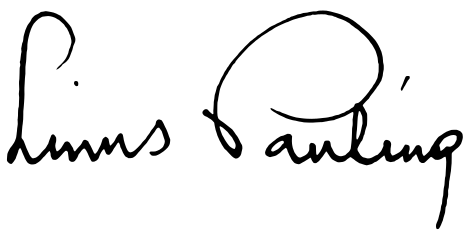
\includegraphics[height=2cm]{coucilsecretarysignature}
    % \end{tabular} &
                      \begin{tabular}{@{}r}
                        \\
                        \councilsecretaryname \\
                        \\
                      \end{tabular}
  \end{tabular}
\end{table}

% \newpage

\resetHeadWidth

% текст введения находится в introduction.tex
% !TEX root = ../synopsis.tex

%
% phdtex
%
% Copyright (c) 2014-2020, Andrew Kanner <andrew.kanner@gmail.com>.
% All rights reserved.
%
% SPDX-License-Identifier: CC-BY-4.0
%

% вынесено из 02-introduction.tex с целью: 1. использования разных
% заголовков в автореферате и тексте диссертации 2. добавления в
% автореферат блока со структурой работы

% нумерация с 3й страницы
\setcounter{page}{3}

% заголовок
\subsection*{\MakeUppercase{Общая характеристика работы}}

% введение
% !TEX root = dissertation.tex

\chapter*{Введение}

% добавляем введение в оглавление
\addcontentsline{toc}{chapter}{Введение}

Текст введения

%\clearpage

% автоматически проставим значения счетчиков из текста диссертации
\getcounter{mychapters}
\getcounter{myappendices}
\getcounter{mypages}
\getcounter{myfigures}
\getcounter{mytables}
\getcounter{mybibitems}

\underline{Структура и объем работы}. Диссертационная работа состоит
из~введения, \themychapters~глав, заключения
и \themyappendices~приложений. Объем основного текста диссертации
составляет \themypages~страниц(ы) с \themyfigures~рисунками
и \themytables~таблицами. Приложение также содержит документы,
подтверждающие практическое использование и внедрение результатов
диссертационного исследования. Количество наименований в списке
литературы --- \themybibitems.

% содержание работы по главам, основные результаты и выводы
% !TEX root = ../synopsis.tex

\subsection*{\MakeUppercase{Основное содержание работы}}

Во \underline{введении} обосновывается актуальность темы
диссертационного исследования, формулируются его цель и задачи,
определяются научная новизна, теоретическая и практическая значимость
полученных результатов. Рассматриваются положения, выносимые на
защиту, апробация и внедрение результатов.

% использовать следующие слова: рассматривается, проводится, показано,
% обосновано, проведен анализ

% \newpage
% ====================================================================

\underline{В первой главе} приводится \dots{}

\dots{}

Таким образом, в главе обоснована актуальность темы диссертационного
исследования, сформулированы постановка научной задачи и возникшее
противоречие, для разрешения которого намечены возможные пути решения
научной задачи исследования и определен состав необходимого
методического обеспечения \dots{}

% \newpage
% ====================================================================

\underline{Вторая глава} посвящена \dots{}

\dots{} какая-нибудь умная формула / график / что-то еще (см. формулу
\ref{test1}) \dots{}

\begin{center}
\begin{equation} \label{test1}
\frac{1}{\Bigl(\sqrt{\phi \sqrt{5}}-\phi\Bigr) e^{\frac25 \pi}} =
1+\frac{e^{-2\pi}} {1+\frac{e^{-4\pi}} {1+\frac{e^{-6\pi}}
{1+\frac{e^{-8\pi}} {1+\ldots} } } }
\end{equation}
\end{center}

Вывод по второй главе.

% \newpage
% ====================================================================

\underline{Третья глава} работы посвящена \dots{}

\dots{} какая-нибудь таблица (см. таблицу \ref{test2}) \dots{}

\setcounter{rowcount}{0}
\captionsetup{belowskip=-10pt}
\begin{longtable}{|c|c|c|}
  \hline

  \textbf{№} & \begin{tabular}{@{}l@{}}\textbf{Текст1} \\
                 \textbf{Текст2}\end{tabular} & Текст3 \\

  \hline
  \endfirsthead

  \multicolumn{3}{|c|}{\small (продолжение таблицы)} \\
  \hline

  \textbf{№} & \begin{tabular}{@{}l@{}}\textbf{Текст1} \\
                 \textbf{Текст2}\end{tabular} & Текст3 \\

  \hline
  \endhead %\hline

  \multicolumn{3}{|r|}{\small (продолжение следует)} \\ \hline

  \endfoot %\hline
  \endlastfoot

  \rownumber & \cellcolor{green!25}Текст & \cellcolor{red!25}Текст \\
  \hline

  \rownumber & \cellcolor{yellow!25}Текст & \cellcolor{green!25}Текст \\
  \hline

  \rownumber & \cellcolor{red!25}Текст & \cellcolor{yellow!25}Текст \\
  \hline

  \caption{Подпись таблицы} \label{test2}

\end{longtable}

Вывод по третьей главе.

% \newpage
% ====================================================================

В \underline{четвертой главе} проводится исследование \dots{}

Вывод по четвертой главе.

% \newpage
% ====================================================================

% !TEX root = ../synopsis.tex

\subsection*{\MakeUppercase{Основные результаты работы}}

\begin{enumerate}

\item Проведен анализ \dots{} исследовано \dots{} предложено \dots{}

\item Сформированы \dots{}.

\item На базе полученных научных результатов разработано \dots{}

\item В ходе экспериментальных исследований подтвержден ожидаемый
  эффект от применения \dots{}, а также соответствие \dots{}.

\end{enumerate}
% основные публикации по теме диссертации
% !TEX root = ../synopsis.tex

%
% phdtex
%
% Copyright (c) 2014-2018, Andrew Kanner <andrew.kanner@gmail.com>.
% All rights reserved.
%
% SPDX-License-Identifier: MIT
%

\subsection*{\MakeUppercase{Список работ, опубликованных по теме
{\tiny }    диссертации}}

\begin{btSect}{parts/biblio-vak-sheet.bib}
%  Статьи в журналах, рекомендованных ВАК для публикаций основных
% результатов диссертационных работ: \btPrintCited
  Публикации в изданиях из перечня ведущих рецензируемых научных
  журналов и изданий ВАК и в изданиях, приравненных к ним: \btPrintAll
\end{btSect}

\begin{btSect}{parts/biblio-scopus-sheet.bib}
%Scopus
  Публикации в изданиях, индексируемых международной системой научного
  цитирования Scopus: \btPrintAll
\end{btSect}

\begin{btSect}{parts/biblio-pub-sheet.bib}
%  Тезисы докладов и материалов конференций: \btPrintCited
  Статьи и материалы конференций: \btPrintAll
\end{btSect}

% \btPrintNotCited \btPrintAll


\end{document}
